\section{Datový model}

Jak již bylo zmíněno výše, datové třídy se nacházejí v adresáři
\verb|core/data|. Aplikace obsahuje celkem 5 datových tříd, z nichž pro každou
je v databázi vytvořena tabulka. Navíc se v datovém modelu ještě nachází
tabulka \verb|config| pro konfiguraci ve formátu \textit{klíč-hodnota}, která je
však v práci použita jen jednou a to pro určení názvu webu, který se nachází
v jeho hlavičce; a tabulka \verb|permissions|, ve které se nacházejí jednotlivá
oprávnění pro skupinu uživatelů.

Tabulka uživatelů se nazývá \verb|users| a obsahuje uživatelská jména,
zašifrovaná hesla, e-maily a odkaz na uživatelskou skupinu, do které daný
uživatel patří.

Každý uživatel musí být po registraci schválen některým z administrátorů.
K tomu slouží tabulka \verb|user_approval|, uchovávající žádosti o schválení.

Tabulka \verb|usergroups| obsahuje tyto uživatelské skupiny. Sestává se pouze
z názvů skupin; oprávnění daných skupin se nacházejí v tabulce
\verb|permissions|, jak je již zmíněno.

Uživatelé mohou nahrávat příspěvky ve formátu PDF. Názvy a abstrakty spolu
s datem vytvoření a modifikace k těmto příspěvkům se nacházejí v tabulce
\verb|article|. Každý článek má rovněž nastaven svůj status, který určuje,
zda článek čeká na schválení či byl přijat nebo zamítnut.

Ke každému nahranému článku mohou recenzenti napsat svou recenzi a navrhnout
administrátorům, zda má být článek přijat, zamítnut, či zda by měl být příspěvek
upraven autorem (a po těchto úpravách přijat administrátory). Všechny recenze
včetně tohoto návrhu se nacházejí v tabulce \verb|review|.

\begin{figure}[h!]
  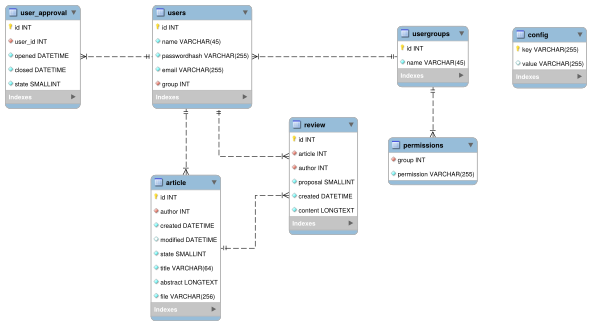
\includegraphics[width=\textwidth]{model.pdf}
  \caption{ER diagram datového modelu}
  \label{fig:erdiagram}
\end{figure}
